\chapter{Eclipse Integration and Testing}
\label{ch:eclipse}

\section{Overview}
After development of the RWU-RV64I software toolchain, the next major step was to integrate it into an efficient and reproducible development environment.  
For this purpose, the \textbf{Eclipse IDE for C/C++ Developers (Eclipse CDT 2023-09)} was used \cite{eclipse-cdt}.  
Eclipse provides a unified interface to write, compile, link, and test C programs targeting the RWU-RV64I processor, using the GNU RISC-V cross-compiler and a Makefile-based project structure.

This integration automates the firmware development cycle — from editing C source files to generating simulation-ready memory files — and eases repeated verification during simulation and FPGA testing (see Chapter~\ref{ch:toolchain} for toolchain details).

% ---------------------------------------------------------------------
\section{Software Requirements}
The following software components were required for complete integration and testing of the RWU-RV64I system:

\begin{itemize}
   \item \textbf{GNU RISC-V Toolchain:} Installed under 
   \texttt{/opt/\allowbreak riscv/}, providing 
   \texttt{riscv64-\allowbreak unknown-\allowbreak elf-\allowbreak gcc}, 
   \texttt{ld}, \texttt{objcopy}, and related utilities 
   \cite{riscv-gnu-toolchain,gcc,binutils}.

  \item \textbf{GNU Make and Binutils:} Used to automate compilation, linking, and conversion steps.
  \item \textbf{Eclipse IDE for C/C++ Developers:} Version 2023-09 (CDT). \cite{eclipse-cdt}
  \item \textbf{Xilinx Vivado Design Suite:} Used for simulation (XSIM), synthesis, implementation, and FPGA bitstream generation. \cite{xilinx-vivado}
  \item \textbf{Zybo Z7-10 Development Board:} The physical platform used for hardware testing. \cite{zybo-datasheet}
\end{itemize}

Toolchain installation can be verified with:
\begin{verbatim}
which riscv64-unknown-elf-gcc
\end{verbatim}

% ---------------------------------------------------------------------
\section{Creating and Importing the Project in Eclipse}
\subsection{Creating a Makefile Project}
\begin{enumerate}
  \item Launch Eclipse → select a workspace directory (e.g. \texttt{~/workspace\_rwu}).
  \item Choose \texttt{File → New → C/C++ Project}.
  \item Select \texttt{Makefile Project with Existing Code}.
  \item Browse to the directory containing the top-level \texttt{Makefile}.
  \item Assign the project name \texttt{rwu-rv64i}.
  \item Under \texttt{Toolchain for Indexer Settings}, select \texttt{Cross GCC}.
\end{enumerate}

\subsection{Disabling Automatic Makefile Generation}
\begin{itemize}
  \item \texttt{Project → Properties → C/C++ Build → Builder Settings}.
  \item Uncheck \texttt{Generate Makefiles automatically}.
  \item Set Build directory to \texttt{\$\{workspace\_loc:/rwu-rv64i/\}}.
\end{itemize}

\begin{figure}[H]
  \centering
  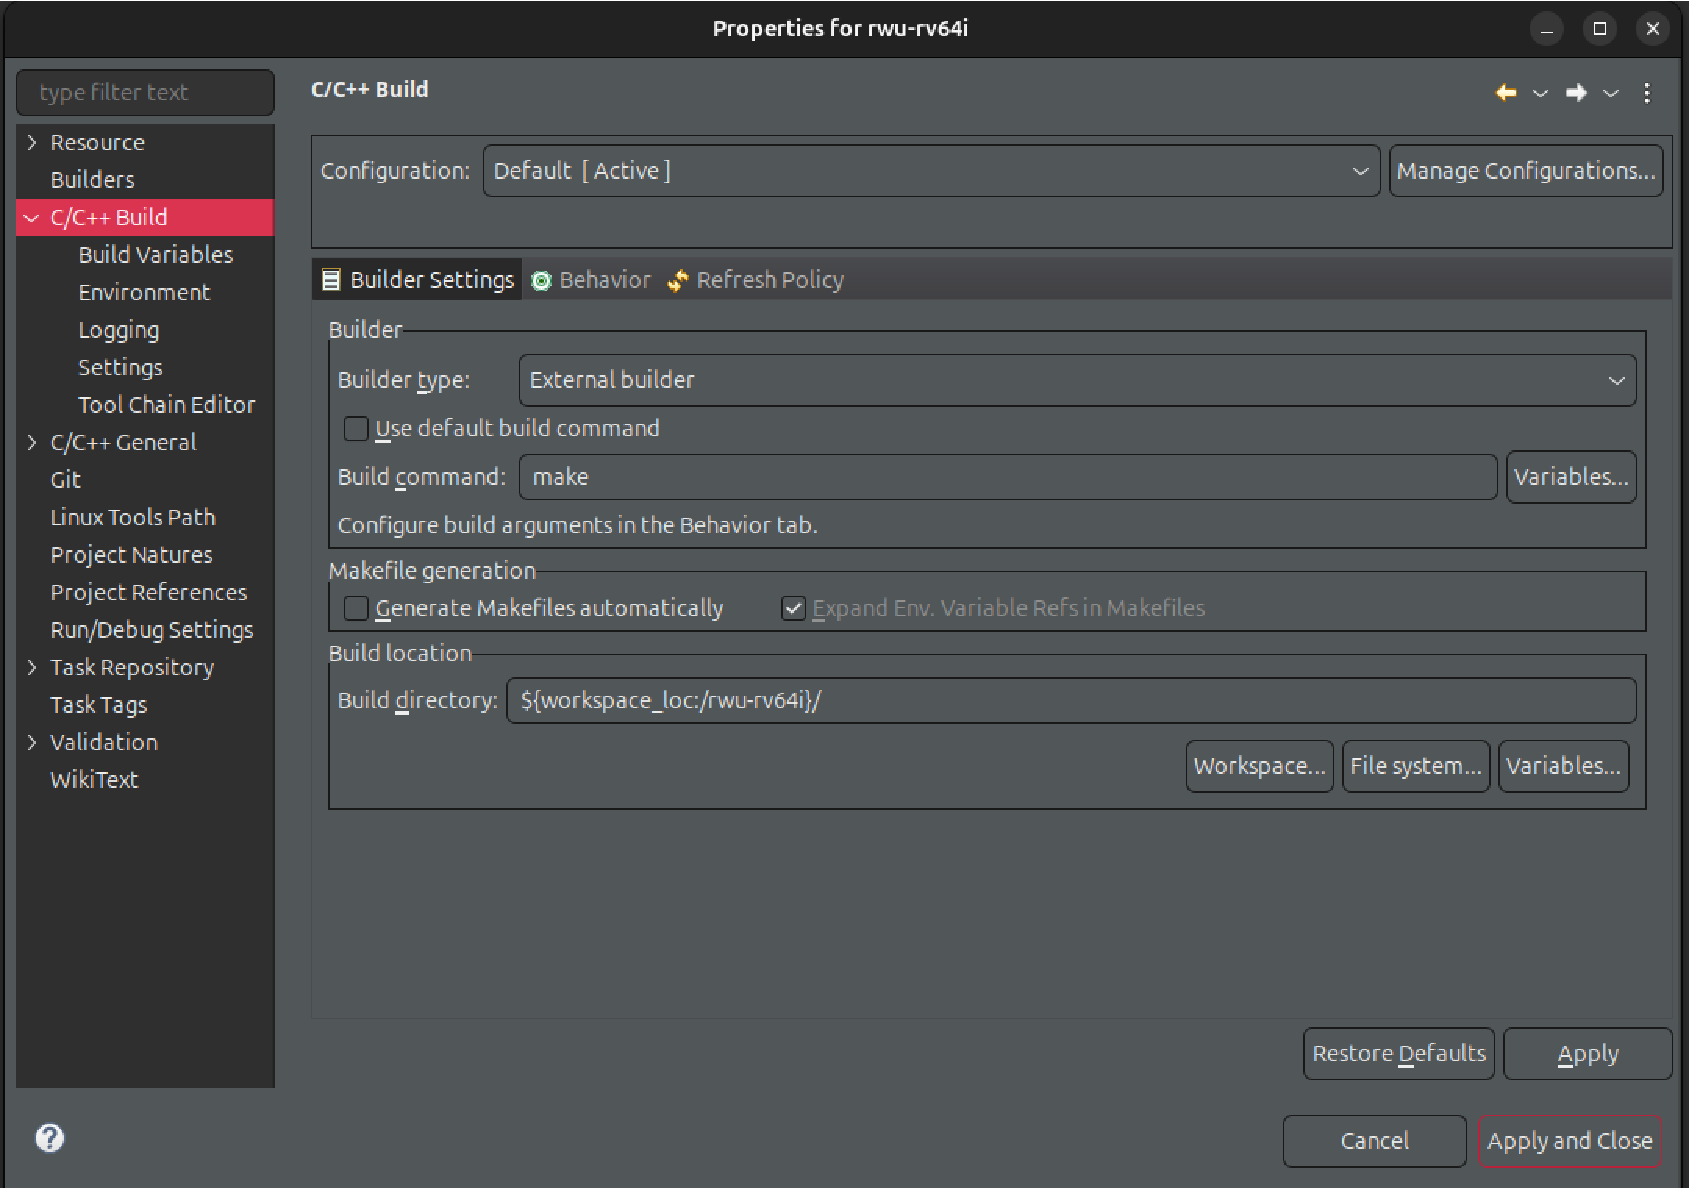
\includegraphics[width=0.9\textwidth]{Thesis_Report/figures/rwu_eclipse_builder.pdf}
  \caption{Eclipse project configuration showing external builder settings.}
  \label{fig:rwu_eclipse_builder}
\end{figure}
% ---------------------------------------------------------------------
\section{Build Environment Configuration}
\subsection{Setting the Compiler Path}
\begin{enumerate}
  \item \texttt{Project → Properties → C/C++ Build → Environment}.
  \item Add environment variable:  
        \texttt{Name: PATH} \texttt{Value: /opt/riscv/bin:\$\{PATH\}}
\end{enumerate}

\subsection{Selecting the External Builder}
\begin{itemize}
  \item \texttt{Project → Properties → C/C++ Build}.
  \item Set \textbf{Builder Type:} \textbf{External Builder}.
  \item Commands:
\begin{verbatim}
Build command: make -j$(nproc)
Clean command: make clean
\end{verbatim}
  \item Working directory: top-level \texttt{Makefile}.
\end{itemize}

\subsection{Defining Make Targets}
Open \texttt{Window → Show View → Other → C/C++ → Make Targets} and define:
\begin{itemize}
  \item \texttt{all}→ \texttt{make all}
  \item \texttt{clean}→ \texttt{make clean}
  \item \texttt{sim}→ \texttt{make sim}
  \item \texttt{waves}→ \texttt{make waves}
  \item \texttt{simcompile}→ \texttt{make simcompile}
\end{itemize}

\begin{figure}[H]
  \centering
  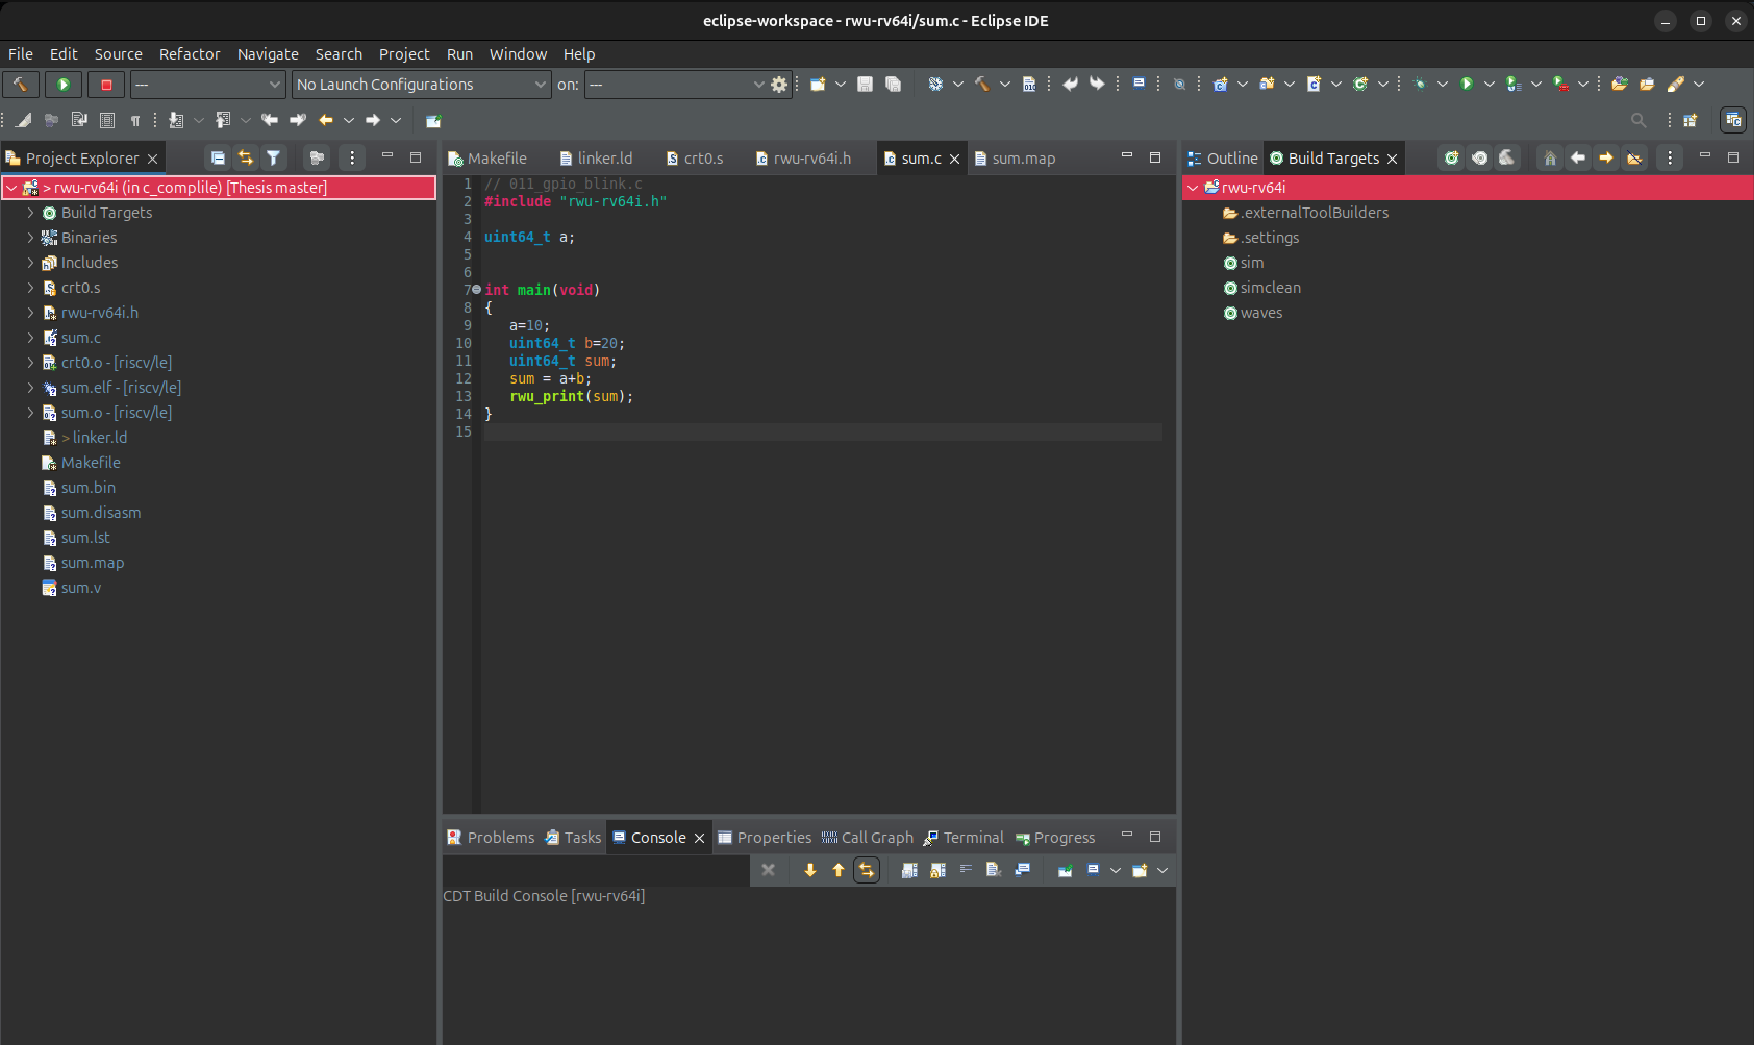
\includegraphics[width=0.9\textwidth]{Thesis_Report/figures/rwu_eclipse_targets.pdf}
  \caption{Make Targets view showing \texttt{sim}, \texttt{simclean}, \texttt{waves} targets.}
  \label{fig:rwu_eclipse_targets}
\end{figure}

These targets enable one-click firmware build, simulation, and waveform analysis.

% ---------------------------------------------------------------------
\section{Makefile Build Process}
The top-level \texttt{Makefile} automates compilation, assembly, linking, and conversion of the program into a Verilog-formatted memory file.  
Only one C source file is compiled per build to simplify traceability.  
The Makefile implementation is included in Appendix~\ref{app:makefile_embedded}.

\subsection{Compilation and Assembly}
C and assembly sources are compiled and assembled using the GNU RISC-V toolchain. The exact flags used by the Makefile are:

\begin{verbatim}
riscv64-unknown-elf-gcc -march=rv64i -mabi=lp64 -ffreestanding \
 -nostdlib -O -g -msmall-data-limit=0 -I. -c program.c -o program.o

riscv64-unknown-elf-gcc -march=rv64i -mabi=lp64 -ffreestanding \
 -nostdlib -O -g -msmall-data-limit=0 -I. -c crt0.s -o crt0.o
\end{verbatim}

\subsection{Linking and Memory Image Generation}
The linker combines the objects using \texttt{linker.ld}, creating the ELF binary:

\begin{verbatim}
riscv64-unknown-elf-gcc -march=rv64i -mabi=lp64 \
 -ffreestanding -nostdlib -T linker.ld crt0.o program.o -o pogram.elf \
 -Wl,-Map=program.map
\end{verbatim}

The ELF file is converted to a Verilog-compatible memory file using:

\begin{verbatim}
riscv64-unknown-elf-objcopy -O verilog program.elf program.v
\end{verbatim}

The output memory file is post-processed and copied into the simulator directory as \texttt{riscvtest.mem} and \texttt{riscvtest\_tb\_sum.mem} (this is automated by Makefile).

\section{Simulation and XSIM Integration}
Simulation is performed in Vivado XSIM. The Makefile invokes the simulator Makefile under \texttt{./sim}, which performs:
\begin{enumerate}
  \item \textbf{Compilation:} \texttt{xvlog --sv} compiles RTL and testbench sources.
  \item \textbf{Elaboration:} \texttt{xelab -debug all} produces an elaborated snapshot.
  \item \textbf{Execution:} \texttt{xsim --runall} runs the simulation using the prepared \texttt{riscvtest.mem}.
\end{enumerate}

The \texttt{waves} target launches the XSIM waveform GUI for signal-level debugging.

\section{Cleaning and Reproducibility}
The Makefile includes cleanup targets:

\begin{itemize}
  \item \texttt{make clean} – removes firmware artifacts (\texttt{.o, .elf, .v, .bin, .lst}).
  \item \texttt{make simclean} – removes simulation outputs (\texttt{.wdb, .log, .xsim.dir}, etc.).
\end{itemize}

These targets ensure that the build is reproducible and that the \texttt{.mem} file always reflects the current firmware.

% ---------------------------------------------------------------------
\subsection{Vivado Project Setup}
A Vivado RTL project was created and populated with:
\begin{itemize}
  \item RWU-RV64I SystemVerilog RTL sources.
  \item The memory initialization file \texttt{riscvtest.mem}.
  \item The constraints file \texttt{Zybo-Master.xdc}.
  \item The top-level module \texttt{as\_top\_mem}.
\end{itemize}

\begin{figure}[ht]
  \centering
  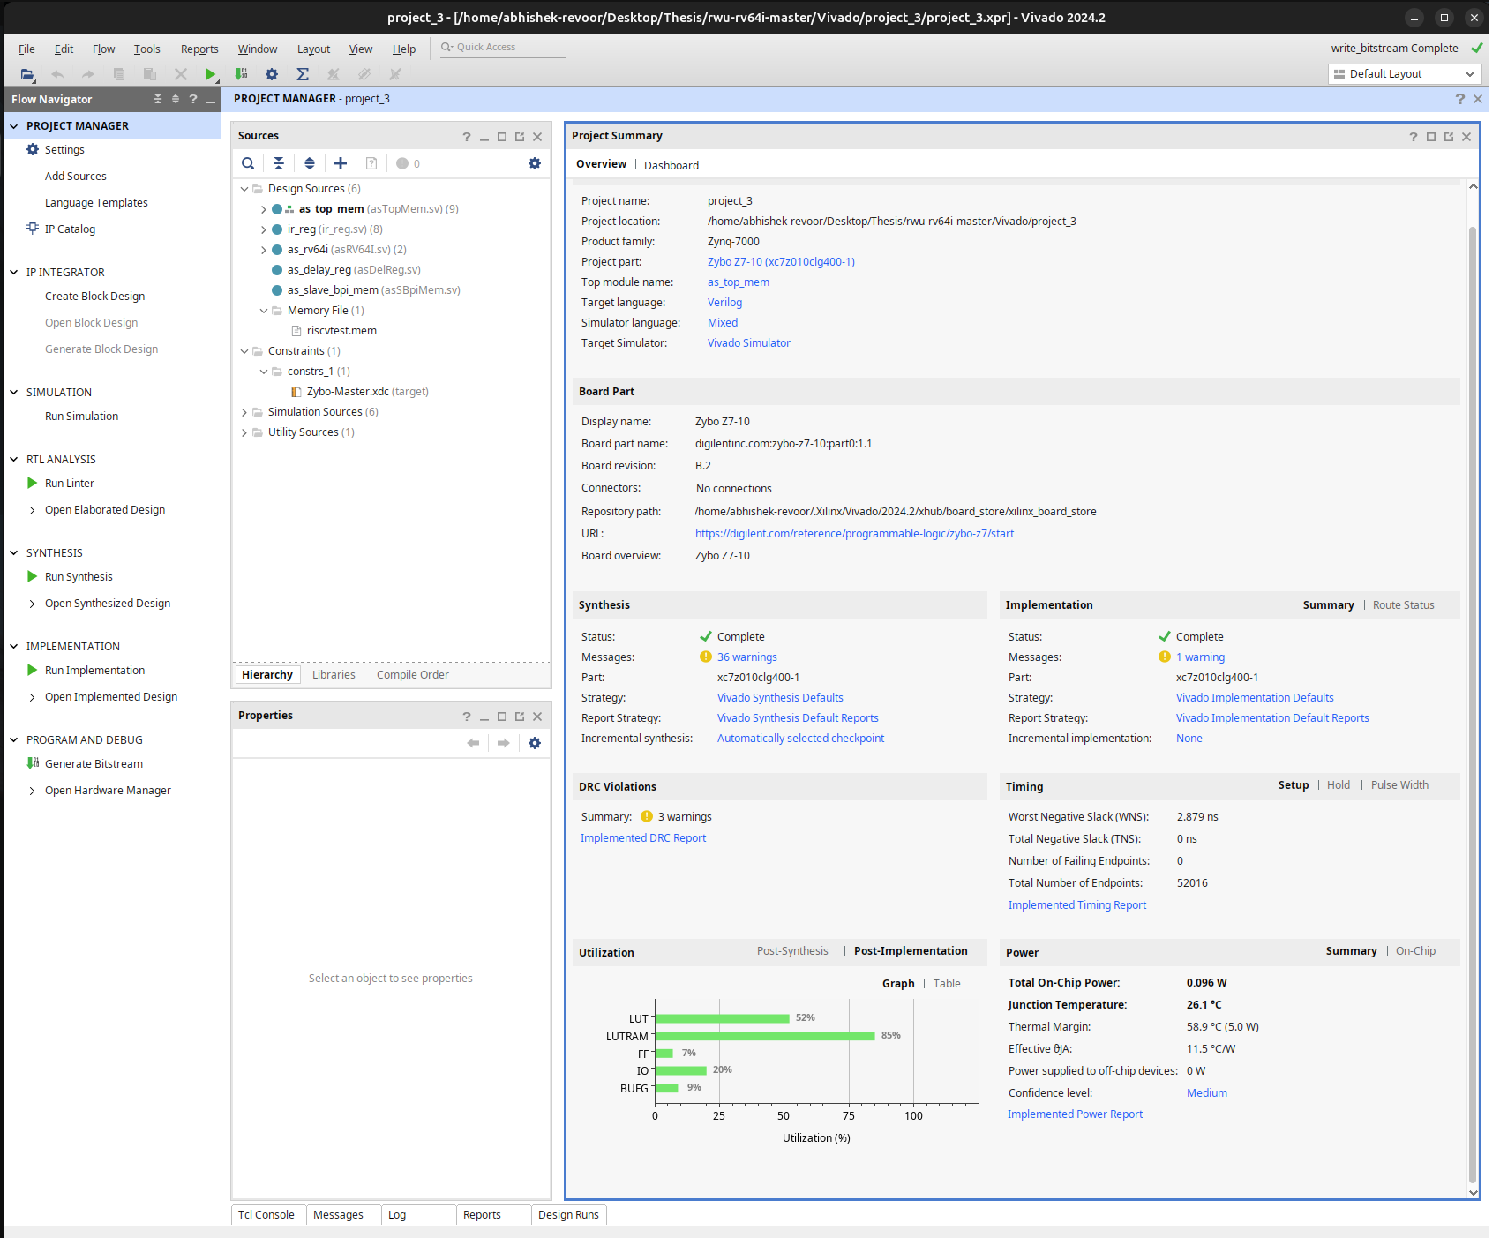
\includegraphics[width=0.9\textwidth]{Thesis_Report/figures/rwu_vivado_project_summary.pdf}
  \caption{Vivado project manager, project summary and source tree.}
  \label{fig:rwu_vivado_project_summary}
\end{figure}

\subsection{Synthesis, Implementation and Bitstream}
The standard Vivado flow (synthesis → implementation → bitstream generation) was executed.  
Vivado inferred both IMEM and DMEM as distributed RAM in this run. For larger images, BRAM inference or explicit BRAM instantiation is recommended to reduce LUT usage.

\begin{table}[H]
  \centering
  \begin{tabular}{lrr}
    \toprule
    Resource & Used & Available \\
    \midrule
    Slice LUTs (total)      & 9,389  & 17,600 \\
    LUT used as logic       & 4,269  & 17,600 \\
    LUT used as memory      & 5,120  & 6,000  \\
    Slice registers         & 2,502  & 35,200 \\
    Block RAM tiles (BRAM)  & 0      & 60     \\
    DSP slices              & 0      & 80     \\
    \bottomrule
  \end{tabular}
  \caption{Key device utilization numbers from Vivado synthesis report.}
  \label{tab:vivado_util}
\end{table}

\subsection{Programming and Running on Board}
To program the Zybo board:
\begin{enumerate}
  \item Connect the board via USB-JTAG.
  \item Open Vivado Hardware Manager and Auto Connect.
  \item Program the device with the generated bitstream.
\end{enumerate}
After programming, the firmware executes from the on-FPGA memories; the test program writes results to the DMEM and the GPIO output, observable via connected LEDs or external probes.

\subsection{Integration correctness}
The toolchain-produced \texttt{riscvtest.mem} was consumed by Vivado and produced the expected runtime behavior on the FPGA. The build and programming sequence executed without critical errors.

\section{Summary}
This chapter described integration of the RWU-RV64I toolchain into Eclipse, the Makefile-driven build and simulation flow, and the FPGA implementation workflow using Vivado.  
The Makefile (see Appendix~\ref{app:makefile_embedded}) enforces a single-C-file workflow and automates the generation of simulation memory images used for both XSIM and FPGA programming.  